\chapter[Hybrid Quantum-Classical Algorithms]{Hybrid Quantum-Classical\\Algorithms} \label{chap:hybrid-quantum-classical-algorithms}
At the end of the previous chapter, two important quantum algorithms were reviewed: the \gls{qft} and Grover's algorithm.
These quantum algorithms and the family of algorithms built on them require large-scale quantum computers with many qubits, low error rates, and high coherence times.
The \gls{nisq} devices that are being built now and in the near future will not be able to run these algorithms due to their limited qubit count, limited coherence times, and high error rates.
To this end, \acrfullpl{hqca} that utilize both classical and quantum resources are being researched and developed.
This chapter will first introduce the basic concepts of an important family of \glspl{hqca} followed by a review of well-known and promising \glspl{hqca}.

\section{Variational Hybrid Quantum-Classical Algorithms}
\Acrlongpl{hqca} take into account the limited number of qubits, limited connectivity of qubits, high error rates, and limited coherence times of \gls{nisq} devices.
These algorithms often make use of the variational method which consists of preparing an initial trial state $\ket{\psi(\vec{\theta})}$ parameterized by real-valued parameters $\vec{\theta}$, and finding the parameters for which the expectation value of some observable is the lowest.
This family of \glspl{hqca} is sometimes also referred to as variational quantum algorithms.
The rest of this chapter will be focused on variational \glspl{hqca}, as this is the main focus of research regarding \glspl{hqca}.

The general structure of a variational \gls{hqca} is shown in \Cref{fig:vqa-general-structure}.
While the specific implementation differs between algorithms, they all share some basic elements.
First, a cost function $C$ which encodes the solution to the problem needs to be defined.
Second, an ansatz needs to be chosen.
The ansatz defines the operations of the quantum circuit which are parameterized by the trainable parameters $\vec{\theta}$.
\begin{figure}[ht]
    \centering
    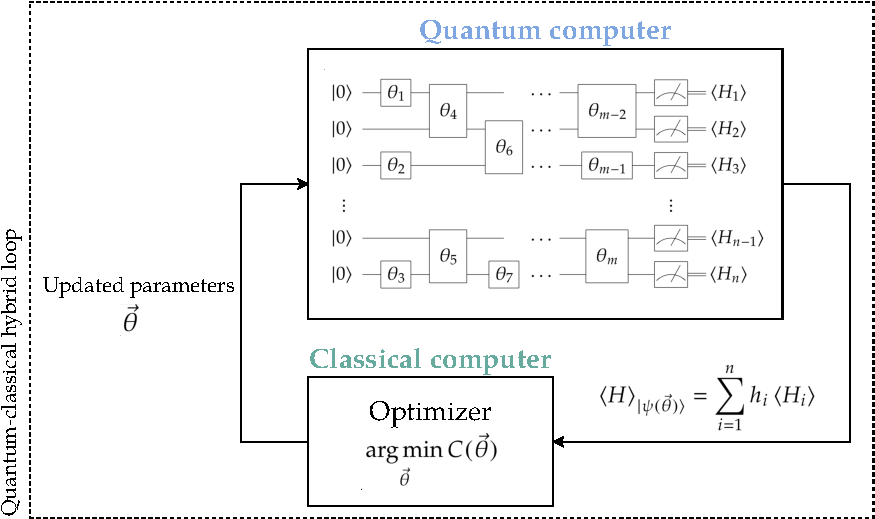
\includegraphics[width=1\linewidth]{figures/vqa-general-structure.pdf}
    \caption[The general structure of a variational \acrshort{hqca}.]{
        The general structure of a variational \gls{hqca}.
        A parameterized quantum state $\ket{\psi(\vec{\theta})}$ is prepared through a set of parameterized quantum gates $U_L(\vec{\theta}_L) \ldots U_2(\vec{\theta}_2)U_1(\vec{\theta}_1)$.
        These parameters are classically optimized according to a cost function $C(\vec{\theta})$.
        This quantum-classical loop is repeated until convergence.
    }
    \label{fig:vqa-general-structure}
\end{figure}
The parameters $\vec{\theta}$ are then trained in a quantum-classical loop to solve the optimization problem
\begin{equation} \label{eqn:optimization-problem}
\vec{\theta}_\text{opt} = \argmin_{\vec{\theta}} C(\vec{\theta}).
\end{equation}

\subsection{Cost Function}
In general, the cost function has the form
\begin{equation} \label{eqn:general-cost-function}
C(\vec{\theta}) = \sum_k f_k\left(\bra{0^n}U(\vec{\theta})^\dagger H_k U(\vec{\theta})\ket{0^n}\right),
\end{equation}
where $f_k$ is a function encoding the problem at hand, $U(\vec{\theta})$ is the quantum circuit parameterized by real values $\vec{\theta}$, and $H_k$ is an observable.
A key point of variational \glspl{hqca} is that a quantum computer is used to estimate $C(\vec{\theta})$ while using a classical computer to optimize the parameters $\vec{\theta}$.
Furthermore, the cost function $C(\vec{\theta})$ should be efficient to estimate by performing measurements on a quantum computer.
For the variational \gls{hqca} to have a quantum advantage, the cost function should also not be efficiently computable with a classical computer.

\subsection{Ans{\"a}tze}
The ansatz defines the quantum circuit $U(\vec{\theta})$ that is used to prepare the quantum state $\ket{\psi(\vec{\theta})}$ parameterized by real-valued parameters $\vec{\theta}$.
To keep the algorithm realizable on \gls{nisq} devices, it is important to keep the parameterized quantum circuit (the ansatz) relatively shallow in depth.
The challenge then is to choose an ansatz that is shallow in depth but has high expressibility.
The expressibility of a quantum circuit is its ability to generate states that are well representative of the Hilbert space~\cite{sim2019expressibility}.
The general form of an ansatz can be described as the product of sequentially applied unitaries:
\begin{equation}
U(\vec{\theta}) = U_L(\vec{\theta}_L) \ldots U_2(\vec{\theta}_2)U_1(\vec{\theta}_1),
\end{equation}
where
\begin{equation} \label{eqn:ansatz-unitary}
U_l(\vec{\theta}_l) = \prod_{m} e^{-i \tfrac{\theta_m}{2} H_m}W_m.
\end{equation}
Here $H_m$ is a Hermitian operator and $W_m$ is a non-parameterized unitary.
\Cref{eqn:ansatz-unitary} can simply be thought of as alternating between parameterized and non-parameterized unitaries.

The specific structure of the ansatz usually depends on the problem, as one can sometimes employ information about the problem to tailor an ansatz~\cite{cerezo2020variational}.
Such ans{\"a}tze are referred to as problem-inspired ans{\"a}tze.
On the other hand, there are problem-agnostic ans{\"a}tze that are used when no information is available for tailoring a specific ansatz.

\subsection{Optimization} \label{sec:optimization}
With the cost function and ansatz defined, the next step in a variational \gls{hqca} is to train the parameters $\vec{\theta}$ using a classical optimization algorithm to solve the optimization problem from \Cref{eqn:optimization-problem}.
The two main types of optimization methods to consider are gradient-based methods and gradient-free methods.
The former methods involve calculating first- or higher-order derivatives of the cost function, while the latter methods use only function evaluations.
In general, the computational cost of gradient-based methods is larger, but the rate of convergence is significantly improved.

While gradient-free methods are straightforward to use for optimizing the quantum circuit parameters, gradient-based methods are more involved.
Consider a parameterized gate of the form $G(\theta) = e^{-i\theta/2 H}$ from the general ansatz description in \Cref{eqn:ansatz-unitary}.
Using the parameter-shift rule as described by \textcite{schuld2019evaluating}, the derivative of the gate $G$ with respect to a parameter $\theta$ can be described as follows:
\begin{equation} \label{eqn:gate-derivative}
\dfrac{\partial G}{\partial \theta} = \dfrac{1}{2}\left[G\left(\theta + \dfrac{\pi}{2}\right) - G\left(\theta - \dfrac{\pi}{2}\right)\right].
\end{equation}
That is, the derivative of $G$ with respect to a parameter $\theta$ can be computed analytically by evaluating the quantum circuit twice with shifted parameters $\theta \pm \pi/2$.

For example, the derivative of a cost function $C(\vec{\theta}) = \sum_k \bra{0^n}U(\vec{\theta})^\dagger H_k U(\vec{\theta})\ket{0^n}$ with respect to a parameter $\theta_l$ can be estimated as follows:
\begin{equation}
\begin{aligned}
\dfrac{\partial C}{\partial \theta_l} = \sum_k \dfrac{1}{2} \bigg[&\bra{0^n}U\left(\vec{\theta} + \dfrac{\pi}{2}\vec{e}_l\right)^\dagger H_k U\left(\vec{\theta} + \dfrac{\pi}{2}\vec{e}_l\right)\ket{0^n} \\
- \; &\bra{0^n}U\left(\vec{\theta} - \dfrac{\pi}{2}\vec{e}_l\right)^\dagger H_k U\left(\vec{\theta} - \dfrac{\pi}{2}\vec{e}_l\right)\ket{0^n}\bigg],
\end{aligned}
\end{equation}
where $\vec{e}_l$ is a vector with $1$ as its $l$-th element and $0$ for all other elements.
Note that calculating $\partial C$ with $m$ parameters $\vec{\theta}$ requires you to evaluate the quantum circuit twice for every parameter, for a total of $2m$ quantum circuit executions per gradient evaluation.
The parameter-shift rule can be further generalized to calculate higher-order derivatives of quantum gates as demonstrated by \textcite{mari2021estimating}, allowing the use of optimization methods that use higher-order derivates such as Newton's method.

A common way to perform gradient-based optimization is through gradient descent based algorithms.
Gradient descent uses first-order derivatives for finding a local minimum of a differentiable function.
Intuitively, it takes repeated steps in the opposite direction of the gradient of the function until the gradient is zero~(\Cref{fig:gradient_descent}).
Formally, for a set of parameters $\vec{\theta}_t$ and a cost function $C(\vec{\theta})$, the updated parameters $\vec{\theta}_{t+1}$ after one iteration of gradient descent are as follows:
\begin{equation}
\vec{\theta}_{t+1} = \vec{\theta}_t - \eta\nabla C(\vec{\theta}_t),
\end{equation}
where $\eta$ is the step size which determines how big of a step the algorithm makes each iteration.
Finding the optimal step size is a practical challenge: if it is too large the optimization algorithm will diverge, and if it is too small it will take a long time to converge.
Methods have been developed to improve the gradient descent algorithm --- for example, the gradient descent based optimization algorithm Adam adapts the step size during optimization to increase the efficiency and accuracy of solutions~\cite{kingma2014adam}.

\begin{figure}[ht]
    \centering
    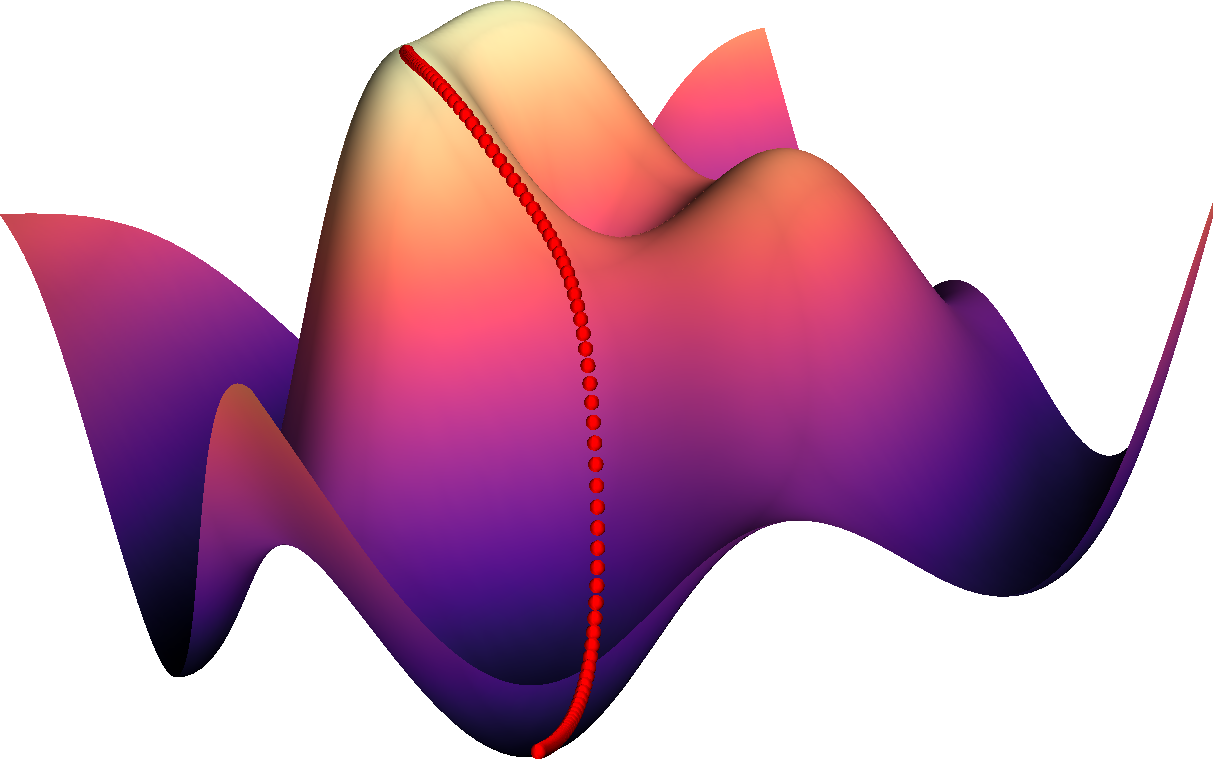
\includegraphics[width=0.45\linewidth]{figures/gradient_descent.png}
    \caption[Visualization of gradient descent finding a local minimum of a function.]{
        Visualization of gradient descent finding a local minimum of a two-dimensional function.
        The red dots represent the value of the cost function at a given iteration.
        The gradient descent algorithm gradually finds a local minimum by moving in the opposite direction of the gradient of the cost function.
    }
    \label{fig:gradient_descent}
\end{figure}

\section{Variational Quantum Eigensolver} \label{sec:vqe}
The \gls{vqe} was the first proposed variational \gls{hqca}.
It aims to solve the problem of finding eigenvalues of a Hermitian matrix $H$.
The problem of finding eigenvalues for large matrices is ubiquitous in quantum chemistry, but potential applications range from determining the results of search engines~\cite{page1999pagerank} to designing new materials and drugs~\cite{golub2000eigenvalue}.
A previously known quantum algorithm called the \acrfull{qpea} solves this problem exponentially faster than the best known classical algorithm~\cite{abrams1999quantum}.
However, the quantum resources required to run the \gls{qpea} greatly exceed the resources available in the near term.
\textcite{peruzzo2014variational} proposed the \gls{vqe} as alternative which can run on \gls{nisq} devices.

Formally, the \gls{vqe} estimates the minimum eigenvalue $\lambda_{\textnormal{min}}$ associated with eigenstate $\ket{\lambda_{\textnormal{min}}}$ for a Hermitian operator $H$.
The cost function is defined as the expectation value of $H$ over a trial state $\ket{\psi({\vec{\theta}})} = U(\vec{\theta})\ket{\psi_0}$ where $U(\vec{\theta})$ is the ansatz and $\ket{\psi_0}$ an initial guess state:
\begin{equation}
C(\vec{\theta}) = \bra{\psi(\vec{\theta})}H\ket{\psi(\vec{\theta})}.
\end{equation}
Minimizing this cost function estimates the minimum eigenvalue of $H$, as the Rayleigh-Ritz variational principle provides the following bound~\cite{ritz1909neue}:
\begin{equation}
\lambda_{\textnormal{min}} \leq \bra{\psi(\vec{\theta})}H\ket{\psi(\vec{\theta})}.
\end{equation}
That is, a trial state $\ket{\psi({\vec{\theta}})}$ will always give an expectation value larger than or equal to the minimum eigenvalue.
In the context of quantum chemistry, where $H$ describes the Hamiltonian of a system, finding the lowest eigenvalue of the Hamiltonian translates to finding the ground state and ground state energy of that system.
By selecting an initial guess state, calculating the expectation value of $H$, and optimizing the cost function $C(\vec{\theta})$, one can then approximate the ground state energy of a Hamiltonian to arbitrary precision.

The problem of estimating the ground state energy is a specific instance of the $k$-local Hamiltonian problem, which looks to find the ground state energy of a $k$-local Hamiltonian.
A $k$-local Hamiltonian is a Hamiltonian that can be expressed as a sum of Hamiltonians $H = \sum_{j}H_j$ where each $H_j$ is a Hermitian operator acting non-trivially on at most $k$ qubits~\cite{bookatz2012qma}.
This problem was shown to be $\QMA$-complete for $k \geq 2$, while the 1-local Hamiltonian problem is in $\P$ \cite{kempe2006complexity}.
However, quantum computers can still offer an advantage above classical computers for this problem.
Any Hamiltonian $H$ can be represented as a linear combination of Pauli operators:
\begin{align} \label{eq:pauli_hamiltonian}
H &= \sum_j h_j P_j \\
  &= \sum_j h_j \prod_k P_j^{(k)},
\end{align} 
where $P_j^{(k)}$ is a Pauli operator $\left\{I, X, Y, Z\right\}$ which acts on qubit $k$, and $h_j$ is a real constant.
From the linearity of quantum observables, it follows that for some state \ket{\psi}
\begin{align}
\melem{\psi}{H}{\psi} &= \sum_j h_j \bra{\psi}P_j\ket{\psi} \\
&= \sum_j h_j \bra{\psi}\prod_k P_j^{(k)}\ket{\psi}.
\end{align} 
The problem of estimating $\melem{\psi}{H}{\psi}$ can be done efficiently on a quantum computer, while being a hard problem to solve classically~\cite{ortiz2001quantum, peruzzo2014variational, kandala2017hardware}.

In order to use the \gls{vqe} to estimate ground state energies of molecules, the energy of the electrons and nuclei in a molecule need to be encoded as a Hamiltonian.
The standard form of such Hamiltonian is as follows:
\begin{equation}
H = - \sum_i \frac{\nabla_{\vec{R}_i}^2}{2M_i}
    - \sum_i \frac{\nabla_{\vec{r}_i}^2}{2}
    - \sum_{i,j} \frac{Z_i}{\lvert\vec{R}_i - \vec{r}_j\rvert}
    + \sum_{i,j>i} \frac{Z_iZ_j}{|\vec{R}_i - \vec{R}_j|}
    + \sum_{i,j>i} \frac{1}{|\vec{r}_i - \vec{r}_j|},
\end{equation}
where $M_i$, $Z_i$, and $\vec{R}_i$ denote the mass, atomic number, and position of nucleus $i$, and $\vec{r}_i$ is the position of electron $i$~\cite{mcardle2018quantum}.
Given the fact that the nuclei are much heavier than the electrons, we can apply the Born-Oppenheimer approximation~\cite{born1927quantentheorie} to separate the Hamiltonian into electronic and nuclear terms.
We are mostly interested in the electronic structure of the molecule, so we can use the Born-Oppenheimer approximation to write the electronic Hamiltonian as
\begin{equation} 
H = - \sum_i \frac{\nabla_{\vec{r}_i}^2}{2}
- \sum_{i,j} \frac{Z_i}{|\vec{R}_i - \vec{r}_j|}
+ \sum_{i,j>i} \frac{1}{|\vec{r}_i - \vec{r}_j|}.
\end{equation}
This form of Hamiltonian is often referred to as the first quantized formulation of quantum chemistry~\cite[Appendix A]{o2016scalable}.
To represent electronic Hamiltonians on a quantum computer, it needs to be mapped from an operator acting on indistinguishable fermions to an operator acting on distinguishable qubits.
There are several approaches to this~\cite{kassal2011simulating}, but the most widely used approach in quantum chemistry uses the second quantized formulation~\cite{mcardle2018quantum}.
The second quantized Hamiltonian must then be mapped into qubits in order to be implemented on a quantum computer.
The most common mappings for this are the Jordan-Wigner~\cite{somma2002simulating} and Bravyi-Kitaev~\cite{seeley2012bravyi} transformations.
The exact details on the different approaches are beyond the scope of this work, but a detailed overview can be found in~\cite{mcardle2018quantum}.

Implementations of the \gls{vqe} can often benefit from using a problem-inspired ansatz.
A popular choice is the \gls{ucc} ansatz, which is a cousin of the coupled-cluster method used in quantum chemistry for describing many-body systems~\cite{shavitt2009many}.
The \gls{ucc} ansatz is parameterized by a polynomial number of parameters, while there is no known efficient classical implementation~\cite{taube2006new}.
Furthermore, the \gls{ucc} ansatz is believed to provide better accuracy than classical coupled cluster methods~\cite{cooper2010benchmark, evangelista2011alternative}.
Despite these advantages, the number of parameters required by the \gls{ucc} ansatz might be too large to allow for practical calculations of large molecules~\cite{wecker2015progress}.
Alternative ans{\"a}tze have been proposed to reduce the quantum resources required for running the \gls{vqe} on larger molecules~\cite{romero2018strategies, kandala2017hardware, grimsley2019adaptive}.

\section{Quantum Approximate Optimization Algorithm} \label{sec:qaoa}
The \acrfull{qaoa} is a variational \gls{hqca} that produces approximate solutions for combinatorial optimization problems~\cite{farhi2014quantum}.
Combinatorial optimization is focused on finding an optimal solution in a finite set of potential solutions.
The number of potential solutions is often too large to scan one by one and select the best option, so more efficient methods are required.
Most combinatorial optimization problems are known to be $\NP$-hard~\cite{schrijver2003combinatorial}.
The \gls{qaoa} depends on an integer $p \ge 1$, for which the quality of the approximation improves as $p$ increases.
Even for $p = 1$, the \gls{qaoa} is not efficiently simulatable by classical computers~\cite{farhi2016quantum}.
The \gls{qaoa} has received attention from the scientific community in the last few years because of its classical intractability, wide range of applications, and promising performance guarantees.

The \gls{qaoa} looks to solve combinatorial optimization problems, which are specified by $n$ bits and $m$ clauses.
A clause is a constraint on a subset of the bits which is satisfied for certain assignment of those bits, and not satisfied for other assignments.
The goal is to find a $n$-bit string $z = \{0,1\}^n$ that maximizes the classical objective function
\begin{equation} \label{eqn:objective-function}
L(z) = \sum_{\alpha=1}^m L_\alpha(z),
\end{equation}
where $L_\alpha(z) = 1$ if $z$ satisfies clause $\alpha$ and $L_\alpha(z) = 0$ if $z$ does not satisfy clause $\alpha$.
The \gls{qaoa} finds a bit string $z'$ for which the approximation ratio $L(z')/L_{\text{max}}$ is large, where $L_{\text{max}} = \max_z L(z)$.
The objective function $L$ can be mapped to a Hamiltonian that is diagonal in the computational basis:
\begin{equation}
H_L = \sum_{\alpha=1}^m H_{L_\alpha},
\end{equation}
where
\begin{align}
H_{L_\alpha} &= \sum_{z \in \{0, 1\}^n} L_\alpha(z) \op{z}{z} \\
&=
\begin{pmatrix}
L_\alpha(0,\ldots,0) & 0 & \cdots & 0 \\
0 & L_\alpha(0,\ldots,1) & \cdots & 0 \\
\vdots & 0 & \ddots & \vdots \\
0 & 0 & \cdots & L_\alpha(1,\ldots,1)
\end{pmatrix}.
\end{align}
The operator $H_L$ encodes the objective function and is referred to as the problem Hamiltonian.

The \gls{qaoa} uses a problem-inspired ansatz which is defined in terms of two alternating unitaries, inspired by the quantum adiabatic algorithm~\cite{farhi2014quantum}.
First, we define a unitary parameterized by $\gamma \in [0, 2\pi)$ using the problem Hamiltonian:
\begin{equation}
U_L(\gamma) = e^{-i\gamma H_L} = \prod_{\alpha=1}^{m} e^{-i\gamma H_{L_\alpha}}.
\end{equation}
Next, we define a mixer Hamiltonian $H_B$:
\begin{equation}
H_B = \sum_{j=0}^{n-1} X^{(j)},
\end{equation}
where $X^{(j)}$ is the Pauli-X gate acting on qubit $j$.
Then, we define a mixer unitary parameterized by $\beta \in [0, 2\pi)$:
\begin{equation}
U_B(\beta) = e^{-i\beta H_B} = \prod_{j=0}^{n-1} e^{-i\beta X^{(j)}}.
\end{equation}
Note that $e^{-i\beta X}$ is just a $R_x(2\beta)$ operation as defined in \Cref{sec:state-evolution}.
Using these unitaries, the ansatz can be described as alternating applications of the problem and mixer Hamiltonian $p$ times using different parameters:
\begin{equation}
U(\vec{\gamma}, \vec{\beta}) = \underbrace{U_B(\beta_p)U_L(\gamma_p) \ldots U_B(\beta_1)U_L(\gamma_1)}_{p \:\, \text{layers}}.
\end{equation}
This unitary depends on $2p$ real parameters $\vec{\gamma} = ( \gamma_1,\ldots,\gamma_p )$ and $\vec{\beta} = ( \beta_1,\ldots,\beta_p )$. 
Note that not all quantum hardware can prepare this ansatz efficiently, so specific hardware-efficient ans{\"a}tze are being proposed \cite{kandala2017hardware, farhi2017quantum}.

Given these definitions, the \gls{qaoa} works as follows.
The system starts in the equal superposition state
\begin{equation}
\ket{s} = H^{\otimes n}\ket{0}^{\otimes n} = \frac{1}{\sqrt{N}} \sum_{j=0}^{N-1} \ket{j}.
\end{equation}
A trial state $\ket{\vec{\gamma}, \vec{\beta}}$ is then obtained by applying the ansatz to \ket{s}:
\begin{align}
\ket{\vec{\gamma}, \vec{\beta}} &= U(\vec{\gamma}, \vec{\beta})\ket{s} \\
&= U_B(\beta_p)U_L(\gamma_p) \ldots U_B(\beta_1)U_L(\gamma_1)\ket{s},
\end{align}
and the cost function to optimize is as follows:
\begin{equation} 
C_p(\vec{\gamma}, \vec{\beta}) = \bra{\vec{\gamma}, \vec{\beta}}H_L\ket{\vec{\gamma}, \vec{\beta}}.
\end{equation}
The subscript $p$ is added to the cost function's definition to indicate the number of layers.
Unlike the \gls{vqe} which minimizes the cost function, we are interested in maximizing $C_p$ to find the bit string which satisfies the most clauses.
We look to solve the optimization problem
\begin{equation}
M_p = \max_{\vec{\gamma}, \, \vec{\beta}} C_p(\vec{\gamma}, \vec{\beta}).
\end{equation}
By measuring $\ket{\vec{\gamma}, \vec{\beta}}$ multiple times in the computational basis we get a bit string $z$ with high probability for which $L(z)$ is near or greater than $M_p$.
The approximation ratio gets better as $p$ increases, and as $p \to \infty$, $M_p = L_{\text{max}}$.
